\documentclass[tikz]{standalone}


\usepackage{tikz}
\usetikzlibrary{calc}

\begin{document}
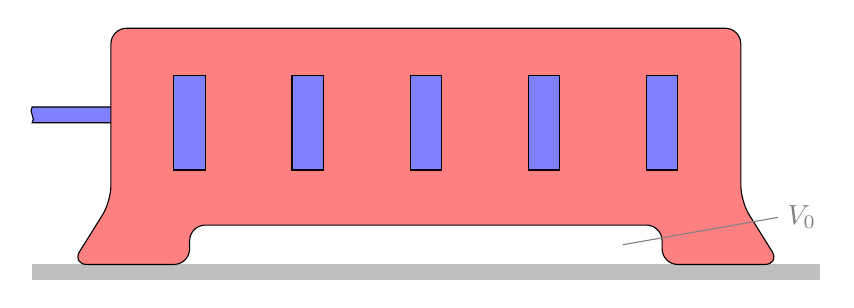
\begin{tikzpicture}[
	scale=1,
	rubber/.style={draw, fill=red!50, rounded corners=2mm},
	air/.style={draw, fill=blue!50},
	substrate/.style={fill=gray!50},
	inlet/.style={draw, fill=blue!50},
	notes/.style={draw, thin, gray}
]

%% Frame

%\foreach \x in {-5,-4, ...,5}{
%	\draw[help lines] (\x,-5)node[below]{\x} -- (\x,5);
%}
%\foreach \y in {-5,-4, ...,5}{
%	\draw[help lines] (-5,\y)node[left]{\y} -- (5,\y);
%}


%% Substrate
\path[substrate] (-5,0)rectangle++(10,-.2);


%% Air Inlet
\path[inlet] (-4,2)--++(-1,0)to[out=-130, in=50]++(0,-.2)--++(1,0);


%% Rubber
\path[rubber] (-4, 3)coordinate(LO)--(-4, .8)--(-4.5, 0)--(-3,0)--(-3, .5)coordinate(LI)
--(3,.5)coordinate(RI)--(3,0)--(4.5, 0)--(4,.8)--(4,3)coordinate(RO) --cycle;
;


%% Air Channels
\def\h{1.2}
\def\b{.4}
\def\hO{1.2}
\foreach \x in {-3, -1.5, 0, 1.5, 3}{
	\path[air] (\x-\b*.5,\hO)rectangle++(\b,\h);
}


%% Notes
\path[notes] (2.5,.25)--++(10:2)node[right]{$V_0$};



\end{tikzpicture}
\end{document}